%From diagram \ref{fig:diagramSystem}, my system has four main blocks. This chapter is dedicated to describe functionalities of these components as well as the background behind.
In this chapter, I present briefly the theoretical background such as Information Extraction and Neural Network. I also discuss related problems like Image Classification, Object Detection as well as their state-of-the-art solutions.

\section{Automatic Speech Recognition}
\label{sec:ASR}
An automatic Speech Recognition (ASR) system is the core part in any voice command system. Given the audio input, the ASR system will output the text form of the input for later processing. Briefly, the audio input is in form of a sound wave over the recording time. It's sampled at a rate of 16000Hz which is enough for recognition. Then this sound wave is chunked at each 20ms and transformed to a spectrogram by using Fourier transform. This is the input (at each time slot) to a recurrent neural network \cite{Medium:2016}. The output at each time slot is recognized characters. After that, a language model is normally used to refine this sequence of characters to a meaningful phrase. 

Note that to build an ASR system that performs at the level of Amazon Alexa or Google Now, we need a lot of training data in both quantity (hundreds of thousands hours of spoken audio) and diversity (native and non-native speakers, with and without background noise). Unfortunately, this kind of data is not available. As the main objective of the project is to use voice to control the robot, not to build a decent ASR system, I decided to use existing software. I explored two solutions: open source systems and Google Cloud.

\subsection{Open-source ASR}
I tried several open-source softwares such as Kaldi \cite{Kaldi:2017}, CMUSphinx \cite{CMUSphinx:2017} and Deep Speech Nervana \cite{DeepSpeech:2017}. As a non-native speaker, I found that they do not perform at an adequate level. For example, I often get "tune rite" when I say "turn right". In addition, it's not easy to use the libraries because long installation processes are required and proper documentation of their usage are limited.

\subsection{Google Cloud Speech API}
My alternative solution is to use a cloud service: Google Speech API \cite{GoogleCloud:2017}. Although the system needs to have internet access, it provides qualitative speech recognition and it is easy to use. We record and sample the audio at 1600Hz, send the signal and get back the recognized text. By using this, we also cut the computation cost of using an ASR server locally. Note that state of the art ASR systems use deep neural network which requires massive computations and resources. For those reasons, I chose to use Google Speech API in my system.

\section{Information Extraction}
\label{sec:InfoExt}
The next task is to extract information from the recognised text. Figure \ref{fig:InfoExt} illustrates this process. Given a command, the most important thing is to know which \tbf{intent} it refers to. Secondly, extract the \tbf{properties} (i.e. parameters) that go with it, such as \textit{direction, quantity, etc.} I explored two solutions for this problem: \tit{Part-Of-Speech (POS) tagging} and \tit{string processing}.

\subsection{Part-Of-Speech Tagging}
Part-Of-Speech tagging is the process of assigning words in the given text to a particular part of speech (such as \tit{noun, verb, adjective, adverb} etc.), based on both word definition and contexts. There are various algorithms to solve POS tagging \cite{Jurafsky:2009:SLP:1214993} and there exist available natural language processing software packages that have a POS tagger embedded, such as NLTK \cite{Loper:2002:NNL:1118108.1118117}, Stanford CoreNLP \cite{manning-EtAl:2014:P14-5}. 

\begin{figure}[tb]
	\centering
	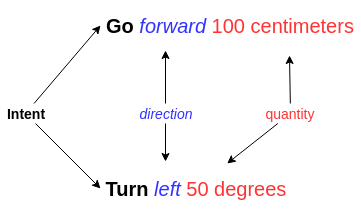
\includegraphics[width=0.6\hsize]{./figures/InfoExt}
	\caption{Illustration of information extraction for movement commands.}
	\label{fig:InfoExt}
\end{figure}

The reason why POS tagging can be helpful is that it classifies words into categories so we can pay attention to key words such as \tit{verbs} (tag VB), \tit{nouns} (tag NN or NNS), \tit{adverb} (tag ADV). For example, the verbs in a command are likely to express \tbf{intent} (turn, move, go, etc.), nouns and adverbs are often \tbf{properties} (left, right, X degrees, Y centimeters, etc.). However, for our specific problem, I found this approach not robust for the following reasons:
\begin{itemize}
	\item There is no perfect POS tagger and its performance depends on its training data. Hence, it did not show good result in tagging command sentences (which hardly appear in a training corpus).
	\item For movement, people tend to use short commands such as: ”backward X metres”, ”turn left” (the angle is 90 degree implicitly). Unfortunately, many of these short commands do not form a complete sentence and POS taggers do not perform well on incomplete sentences.
\end{itemize}
Figure \ref{fig:POSTagLimits} illustrates the above idea. For example, POS tagger predicts word \tbf{turn} as a noun instead of a verb, and predicts word \tbf{left} as a verb in past tense instead of an adverb. Such misclassifications are frequent and they make the system vunerable. That's the reason why I switched to the alternative approach: string processing.

\begin{figure}[tb]
	\centering
	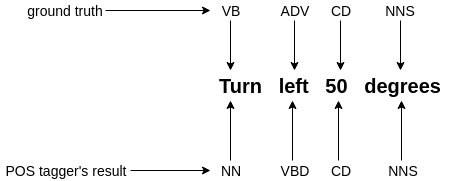
\includegraphics[width=0.7\hsize]{./figures/POSTagLimits}
	\caption{Limitation of POSTaggers: it does not perform well on sentences that describe commands or orders since those hardly appear in training corpus.}
	\label{fig:POSTagLimits}
\end{figure}

\subsection{String Processing}
Instead of tagging words to categories and dealing with key words (verbs, adverbs, nouns), I just analyse the text by the following steps:
\begin{itemize}
	\item Remove redundant words (please, so, well)
	\item Define a synonyms set for my problem and replace synonym words by its representative. For example: \tit{go, move, travel} all map to \tit{go}; \tit{turn, rotate, spin} all map to \tit{turn}; \tit{right, right-side} all map to \tit{right} and so on. By doing this, I have limited and specific words describing \tbf{intent} and \tbf{direction}.
	\item Search for intent words, the directions and check for words describing quantities. Those tokens are in digit format and normally appear at fixed positions corresponding to current intent.
\end{itemize}

This approach is simple but it works robustly and consistently for our specific information extraction problem.

\section{Neural Network Overview}
\label{sec:neuralNet}
The use of a neural network is a key technique behind many artifical intelligent systems today. Although there was much research on neural network in the later part of the 20th century \cite{Bishop:1995:NNP:525960} this paradigm for artificial intelligence has only dominated in recent years (since 2012) mainly because of the availability of large datasets and powerful computation units (strong graphics processing units (GPUs)). This section presents briefly fully connected and convolutional neural networks which perform best in image classification. For a more rigorous treatment, see books such as Deep Learning \cite{Goodfellow-et-al-2016}, or chapter 5 of Pattern Recognition and Machine Learning \cite{Bishop:2006:PRM:1162264}.
\subsection{Fully-connected Neural Network}
In supervised learning, a fully-connected neural network is usually used as an classifier (which computes probability that an input data is as an instance of each of a finite set of classes). More precisely, a fully-connected neural network is a directed graph that comprises an input layer, a sequence of hidden layers and an output layer, where each node in each layer has a link (with weight and bias) to each node in the next layer. Therefore, each output node has potential contribution from each input node and for an image classification problem, each contribution will be \tit{trained} during training process to give some measure that an input is of a unique class. An example is shown in figure \ref{fig:fcNet}: The input data is presented by the input layer (such as vector of image features) and is passed forward through the network to the output layer which represents the probabilities of input's labels. Between each layers, there are learnable parameters: matrix \textbf{weight $W$} and vector \textbf{bias $b$}. Look at figure \ref{fig:fcNet}, we can see that $h = W_1 x + b_1$. Intuitively, we can think of the bias vector as the constant slope added to make $h$ more flexible. After that, we add nonlinearity to the network by applying an activation function $f(h) = max(h, 0)$. In practice, it is up to us to choose the number of hidden layers and theirs sizes. 

For each specific problem, a loss function (or multiple loss functions) will be defined accordingly to help train the network by penalising wrong predictions. For better understanding, assume that we are solving a classification problem. Briefly, during training, input is passed \tbf{forward} through the network and categorical probabilities are computed at the last layer. If this predicted distribution is wrong then the loss is high. We compute the derivatives of the loss w.r.t previous layer and pass these derivatives \tbf{backward}. In backward pass, we update the parameters (weight and bias) in order to \tbf{minimise the loss}. This forward and backward pass is repeated many times on training data to train the network (i.e. update the parameters) until we observe that the loss does not decrease anymore. Now the network has learnt and is ready to predict the class of a never-seen input. We will discuss more about this in subsections \ref{subsec:loss} and \ref{subsec:trainRegime}. 
%Based on the dimensions of input features, number of classes, and hidden layers' sizes, we can easily determine the dimension of these parameters. 
\begin{figure}[tb]
	\centering
	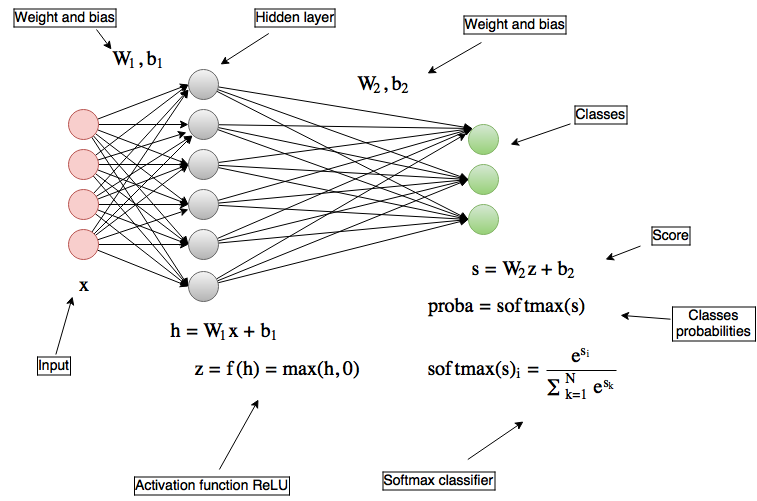
\includegraphics[width=0.9\hsize]{./figures/fcNet}
	\caption{A simple fully connected neural network which classifies an input data into 3 categories using softmax classifier and rectified linear unit activation function (ReLU).}
	\label{fig:fcNet}
\end{figure}
In practice, fully-connected layers are combined with other blocks. For example, figure \ref{fig:convNet1} shows a simple convolutional neural network with a fully-connected layer placed at the end to classify the input image.
\begin{figure}[tb]
	\centering
	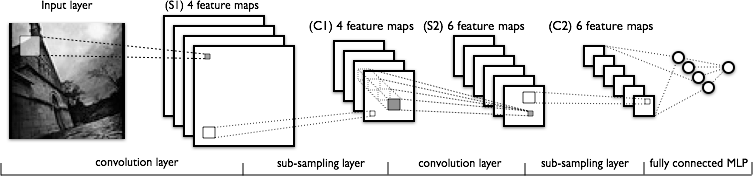
\includegraphics[width=0.9\hsize]{./figures/convNet1}
	\caption{A simple convolutional neural network: its neurons are transposed into 3D shape (width, height and depth) at each layer. The fully connected layer is placed at the end to classify input. Image source: \cite{deeplearningTut}}
	\label{fig:convNet1}
\end{figure}
\subsection{Convolutional Neural Network}
A Convolutional Neural Network (CNN) is designed to solve problems that take images as input. Intuitively, since convolution is a fundamental filtering operation applied on images to preprocess or to extract interesting information, people came up with the idea of stacking many filters (to form \tit{convolutional layers}) together to build good features from raw images. We can also see that convolutional layers are similar to an animal's visual cortex, where an individual neuron may respond to only a small region of the visual field and successive layers are characterised by a distinctive structure associated with more aggregate feature extraction.

Next, we input these features to a fully-connected neural network (for example to classify images into a finite set of classes). In general, when we talk about a convolutional neural network, we also mean that the fully-connected layers is plugged at the end. 

Image inputs usually have a 3D shape: width, height and 3 color channels (RGB). Hence, convolutional neural network also aranges its neurons in 3 dimensions: width ($w$), height ($h$), depth ($h$). Note that the depth of input layer equals the number color channels of input image and the \textbf{depth of convolution layer equals the number of filters applied at that layer}. If we use filters of size $3*3$, then in a convolutional layer $i$:
\begin{itemize}
	\item the weight $W_i$ is a stack of filters and it contains $dim(W_i) = 3 \times 3 \times d_{i-1} \times d_i$ parameters where $d_{i-1}$, $d_i$ are depth of the previous layer $i-1$ and the current layer $i$ respectively. We can explain the dimension of $W_i$ as follows:
	\begin{itemize}
		\item input to the current layer $i$ has the dimension $w \times h \times d_{i-1}$ 
		\item convole (with padded zeros to maintain the same width and height) one filter of dimension $3 \times 3 \times d_{i-1}$ with that input will output $w \times h \times 1$ tensor (\tit{tensor is the terminology for multi-dimensional array}). In order to get an output of dimension $w \times h \times d_i$, we will need $d_i$ such filters. Therefore, weight $W_i$ has $dim(W_i) = 3 \times 3 \times d_{i-1} \times d_i$.
	\end{itemize}
	\item the bias $b_i$ is the vector with length equals number of filters, i.e. $b_i \in R^{d_i}$. At each depth level $k \in \{1, 2, ..., d_i\}$, output tensor (the k-th slice $w\times h$) is added element-wise the amount $b_{i_{k}}$.

	\item We apply activation function ReLU: $f(h) = max(h, 0)$ to the current tensor.
	\item We optionally sub-sample the current tensor to keep strongest features and reduce tensor size. Normally $w_{new} = w / 2$, $h_{new} = h/2$. We have the output tensor of size $w_{new} * h_{new} * d_i$ that will be passed to next layer $i+1$.
\end{itemize}  
The process is illustrated in figure \ref{fig:convNetsimple}. And a common method for sub-sampling called \tbf{max-pooling} shown in figure \ref{fig:maxpool}. It partitions each "slice" of the tensor into non-overlapping rectangles and choose the maximum value in each rectangle. Hence, we produce non-linearities and prioritise strongest features.
\begin{figure}[tb]
	\centering
	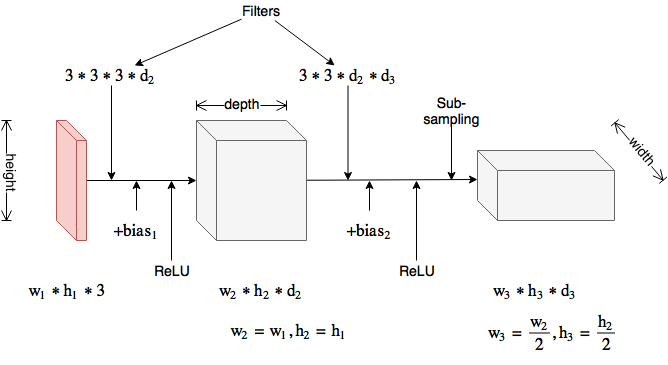
\includegraphics[width=0.9\hsize]{./figures/convNetsimple}
	\caption{Operations and parameters of convolution layers. Note that only input image and 2 convolution layers are drawn here.}
	\label{fig:convNetsimple}
\end{figure}
\begin{figure}[tb]
	\centering
	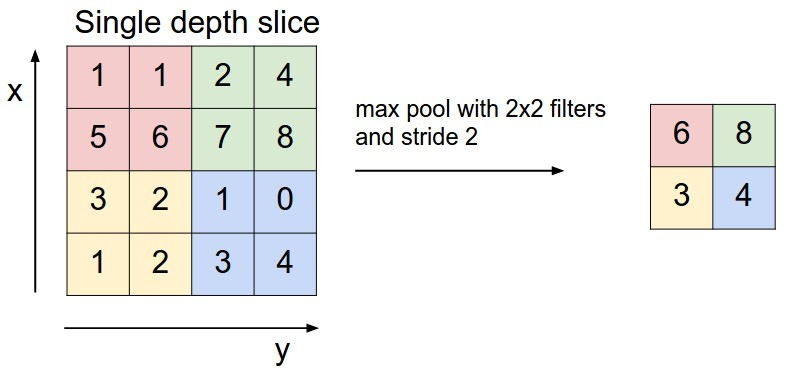
\includegraphics[width=0.6\hsize]{./figures/maxpool}
	\caption{Max-pooling to reduce tensor size and keep strongest features. Image source: \cite{cs231n}}
	\label{fig:maxpool}
\end{figure}

After several convolution layers, we flatten the tensor to put into a fully connected neural network for classification. Note that at these fully connected layers, we often use \textbf{dropout} which is a technique to reduce overfitting at fully connected layers because most of parameters present at these layers (figure \ref{fig:dropout}). In training time, we have a probability (normally $p=0.5$) of dropping out neurons in the fully connected layers from the network and then reinsert the dropped out nodes. We repeat that process for every forward and ackward pass. This will also bring a similar effect as model ensemble. In addition, dropout technique can also be used at convolution layers. For more detail about dropout, please refer to \cite{Srivastava:2014:DSW:2627435.2670313}.
\begin{figure}[tb]
	\centering
	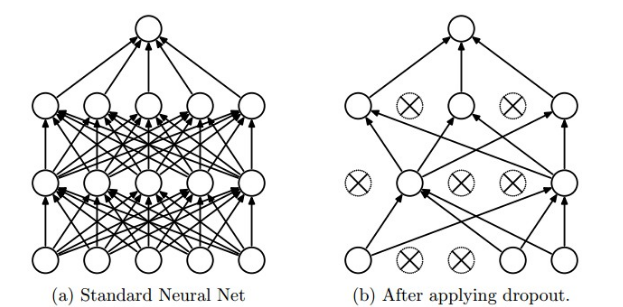
\includegraphics[width=0.8\hsize]{./figures/dropout}
	\caption{Dropout helps to reduce overfitting and ensemble models. Image source: \cite{Srivastava:2014:DSW:2627435.2670313}}
	\label{fig:dropout}
\end{figure}

\subsection{Loss Function}
\label{subsec:loss}
We are left to define a loss function: which allows us to train a machine learning model by updating parameters in order to minimise loss. For classification problems we often use the popular cross-entropy loss function. Consider an input indexed $i$, then its cross-entropy loss is
\begin{align}
\label{form:CELoss}
L_i = -\log(\frac{e^{s^{(i)}_{y_i}}}{\sum_{k=1}^{N}e^{s^{(i)}_k}}) = -s^{(i)}_{y_i} + \log\sum_{k=1}^{N}e^{s^{(i)}_k}
\end{align}
where $y_i$ is its ground-truth label, $s^{(i)}$ denotes its score at the last layer and $N$ is the number of classes (see figure \ref{fig:fcNet}). We can see from formula (\ref{form:CELoss}) that if the score for ground-truth label gets bigger then the loss gets smaller. Next, for each iteration, we apply formula (\ref{form:CELoss}) on a batch of training data $B$ (of cardinal $|B|$):
\begin{align}
L_B = \frac{1}{|B|}\sum_{i \in B} \bigg(-s^{(i)}_{y_i} + \log\sum_{k=1}^{N}e^{s^{(i)}_k}\bigg)
\end{align}
and use stochastic gradient descent \cite{wiki:SGD} to update the parameters accordingly:
\begin{align}
W^{(n+1)}_i &= W^{(n)}_i - \alpha \frac{\partial L_B}{\partial W^{n}_i}\\
b^{(n+1)}_i &= b^{(n)}_i - \alpha \frac{\partial L_B}{\partial b^{n}_i}
\end{align}
where $W_i, b_i$ are parameters of the model (weights and biases), $n$ denotes number of iteration and $\alpha$ is learning rate - a hyperparameter of the model. The gradients are computed by algorithm back-propagation. For more details, please refer to Deep Learning \cite{Goodfellow-et-al-2016} or chapter 5 of Pattern Recognition and Machine Learning \cite{Bishop:2006:PRM:1162264} or Wikipedia \cite{wiki:backpropagation}.

\subsection{Train, Validate and Test regime}
\label{subsec:trainRegime}
To train and validate a machine learning model, we usually split the dataset into 3 parts: training set ($\approx56\%$), validation set ($\approx14\%$) and test set ($\approx30\%$). We will use training dataset to train the model (in our case they are all the parameters $W_i$, $b_i$) and use the validation dataset to tune other hyperparameters: learning rates, dropout probability, hidden layer sizes, number of filters etc. Once we have done our best on the validation set, we run the model only once on the test dataset to obtain the test accuracy. This figure will be our model performance. 

\section{Image Classification}
\label{sec:imgClass}
\subsection{Problem Description}
\textbf{Image Classification} is the task of assigning an input image to one label from a fixed set of categories. It is directly related to the object finding problem. We will discuss further this point in section \ref{sec:objDetect}. Although the description is short, it is really challenging to achieve a high accuracy ($\geq$ 90\%) because of the following difficulties (figure \ref{fig:ImClasschallenges}):
\begin{enumerate}
	\item Viewpoint variation: the same object can be captured at different camera positions.
	\item Illumination conditions: computers only see the pixel values and minor changes in illumination can result in totally different pixel values. 
	\item Scale variation: the same object can have different sizes in the real world. In addition, the distance of taking photo also cause this variation.
	\item Deformation: many objects are not static hence their forms are never unique.
	\item Occlusion: depend on the camera view, sometimes only a portion of object is visible.
	\item Background clutter: when object and background are similar
	\item intra-class variation: there are many different types and styles of the same object class (e.g. keys, chairs)
\end{enumerate}

\begin{figure}[tb]
\centering
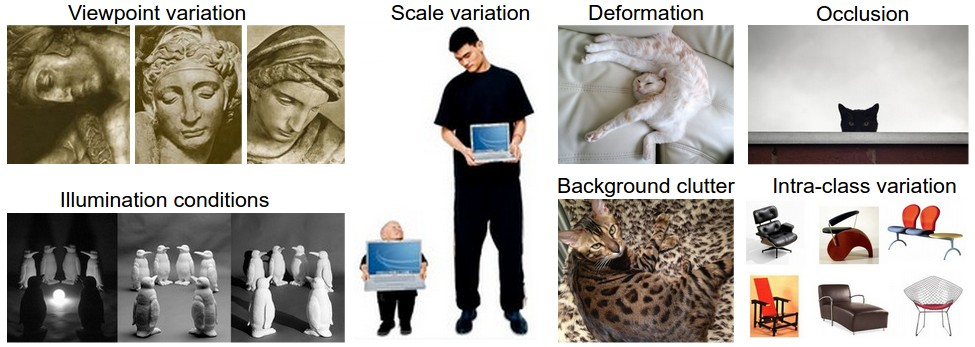
\includegraphics[width =0.9\hsize]{./figures/ImClasschallenges}
\caption{Some challenges of Image Classification problem. Image source: \cite{cs231n}.}
\label{fig:ImClasschallenges}
\end{figure}
\subsection{A State-of-the-art Solution}
Each year, there is an ImageNet Large Scale Visual Recognition Competition (ILSVRC) \cite{ILSVRC15} where research groups from around the world participate and submit their state of the art solution to multiple visual recognition problems. Image Classification is only one task in the challenge. There are 2 evaluations for this task: the top-1 and top-5 accuracies. \tbf{Top-\tit{n} accuracy is the rate that your top \tit{n} predictions (i.e. the \tit{n} ones with highest probabilities) contain the ground truth label}. In addition, people also use the term top-\tit{n} error rate, which is defined as follows: 
$$ \text{Top-\tit{n} error rate} = 1 - \text{Top-\tit{n} accuracy}$$
Please note that, for this task, human beings achive only 5.1\% top-5 error rate, which equals to 94.9\% top-5 accuracy. Since 2012, the best solutions for image classification are always deep convolutional neural networks (CNNs). Figure (\ref{fig:imagenetTop5Err}) illustrates this point. Given the fundamental notions represented in section \ref{sec:neuralNet}, I restate below a brief explaination for the success of CNNs:
\begin{itemize}
	\item Deep neural networks accomodate non-linearity properties through activation layers. This makes the system more flexible and able to prioritise important features.
	\item Each convolutional layer is a stack of filters. After learning (i.e. at test time), those filters can extract from input image many types of features such as: edge, shape, colors etc. (for more details please refer to \cite{DeepVis:2015})
	\item Convolutional layers act as features builder, and given enough data, machines do this job better than human beings (from figure \ref{fig:imagenetTop5Err}, we can see that ResNet with 152 layers reaches 3.6\% top-5 error rate).
\end{itemize}
In my experiment, I explored the following models:
\begin{itemize}
	\item VGG16 \cite{DBLP:journals/corr/SimonyanZ14a} - a model of VGG group from Oxford University, one winner of ImageNet competition in 2014.
	\item Resnet50 \cite{DBLP:journals/corr/HeZRS15} - a model from Microsoft research group, winner of ImageNet competition in 2015.
	\item Xception \cite{DBLP:journals/corr/Chollet16a} - a model based on GoogleNet \cite{DBLP:journals/corr/SzegedyVISW15} (winner of ImageNet competition in 2014).
\end{itemize}
Overall, Resnet50 performs the best with better accuracy and shorter computational time.

\begin{figure}[tb]
\centering
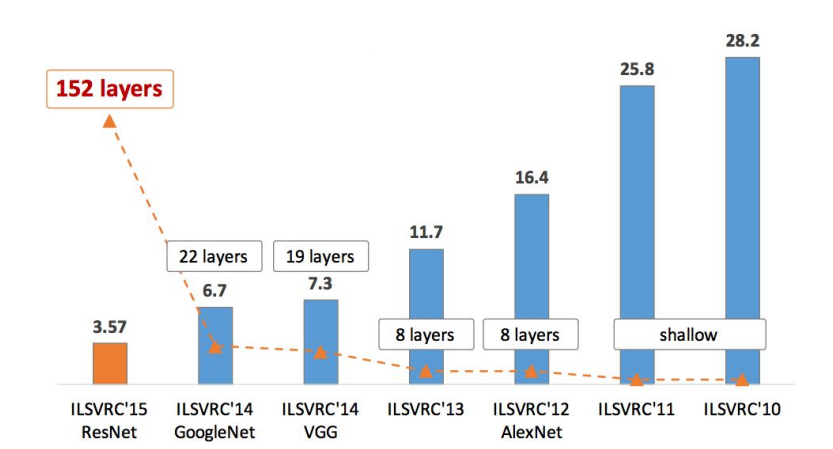
\includegraphics[width=0.8\hsize]{./figures/imagenetTop5}
\caption{Top 5-error rate in Imagenet Classification competition from 2010 to 2015. We can note a huge improvement from traditional approaches which use hand-crafted computer vision features (2010, 2011) to deep convolutional neural network (2012). VGG model \cite{DBLP:journals/corr/SimonyanZ14a} is one of the winners in 2014. Its performance nearly equals human beings (5.1\%). Resnet model \cite{DBLP:journals/corr/HeZRS15} is the winner in 2015. \tit{Figure copyright Kaiming He.}}
\label{fig:imagenetTop5Err}
\end{figure}

\subsection{Transfer Learning}
\label{sec:transferLearning}
Transfer Learning is a technique in Machine Learning where knowledge gained during training in one type of problem is used to train in other similar problems. This helps save time and resource by avoiding training a model from scratch. The technique is extensively used for deep neural network models because these normally have a lot of parameters and training from scratch can take weeks. Therefore, to solve our image classification problem, I applied transfer learning on the 3 models discussed in previous subsection. The transfer learning process for image classification problem (figure \ref{fig:transferLearning}) is described as following:
\begin{enumerate}
	\item Initialize the model by using its pretrained weights and biases. Those parameters are provided by their authors.
	\item Cut and replace the fully connected layers of the original model by our \tit{appropriate} fully connected layers. For example, original models classify 1000 objects but our has only 12 categories to classify.
	\item Freeze all layers in convolutional blocks and start training new fully connected layers for a while (10-20 epochs).
	\item Unfreeze final convolutional layers and start fine-tuning model (i.e. training with smaller learning rate).
\end{enumerate}

\begin{figure}[tb]
	\centering
	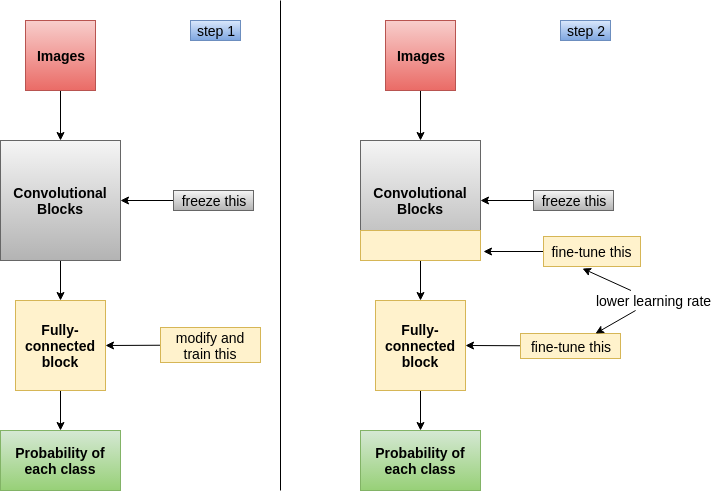
\includegraphics[width=0.9\hsize]{./figures/transferLearning}
	\caption{Transfer Learning process}
	\label{fig:transferLearning}
\end{figure}

Remember that our problem is to classify objects belongs to 12 categories: \tit{"apple", "pen", "book", "monitor", "mouse", "wallet", "keyboard", "banana", "key", "mug", "pear", "orange"}. They are ordinary things that we see and use daily. To form the dataset, I downloaded 1200 images for each category from ImageNet \cite{imagenet_cvpr09}.

The original VGG16 model is shown in figure \ref{fig:originalVgg16} with details about tensors and filters' shape. On the other hand, one example of applying transfer learning on VGG16 is shown in figure \ref{fig:transferedVgg16}. In this example, we modified the fully connected part and did not fine-tune the final convolutional block. Experimental results about fine-tuning will be given in chapter \ref{chap:ExpRes}.
\begin{figure}[tb]
	\centering
	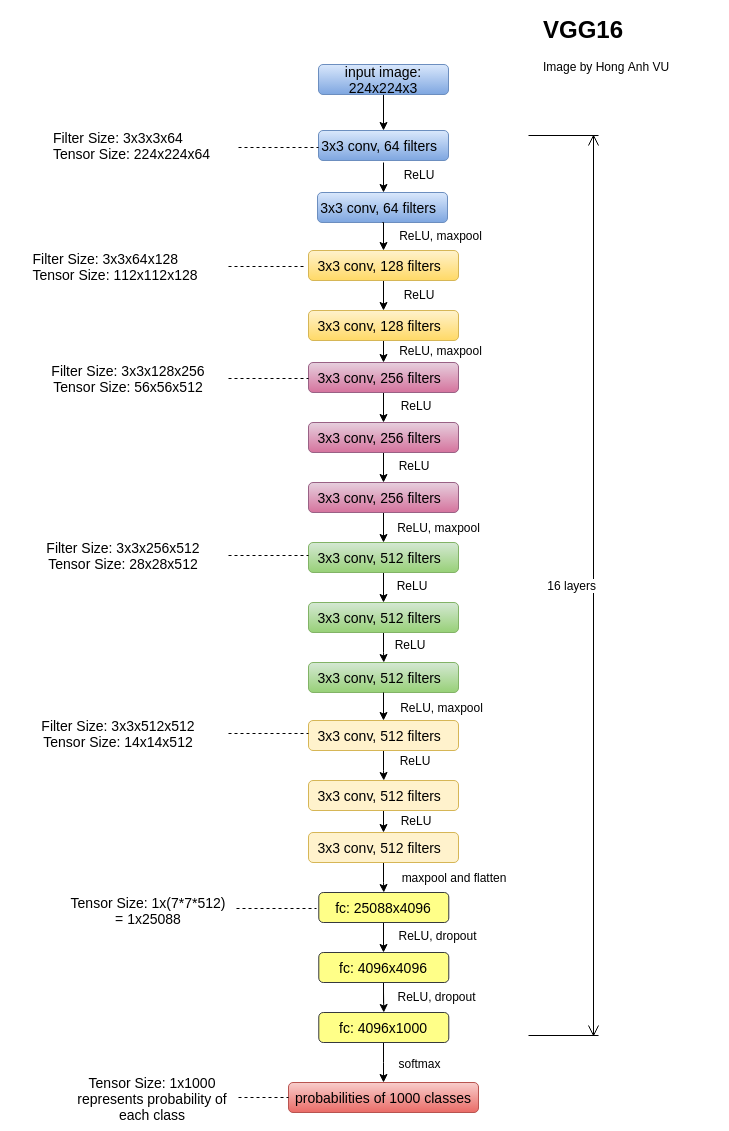
\includegraphics[width=0.9\hsize]{./figures/originalVgg16}
	\caption{Original VGG16 model. There are 1000 categories to classify.}
	\label{fig:originalVgg16}
\end{figure}

\begin{figure}[tb]
	\centering
	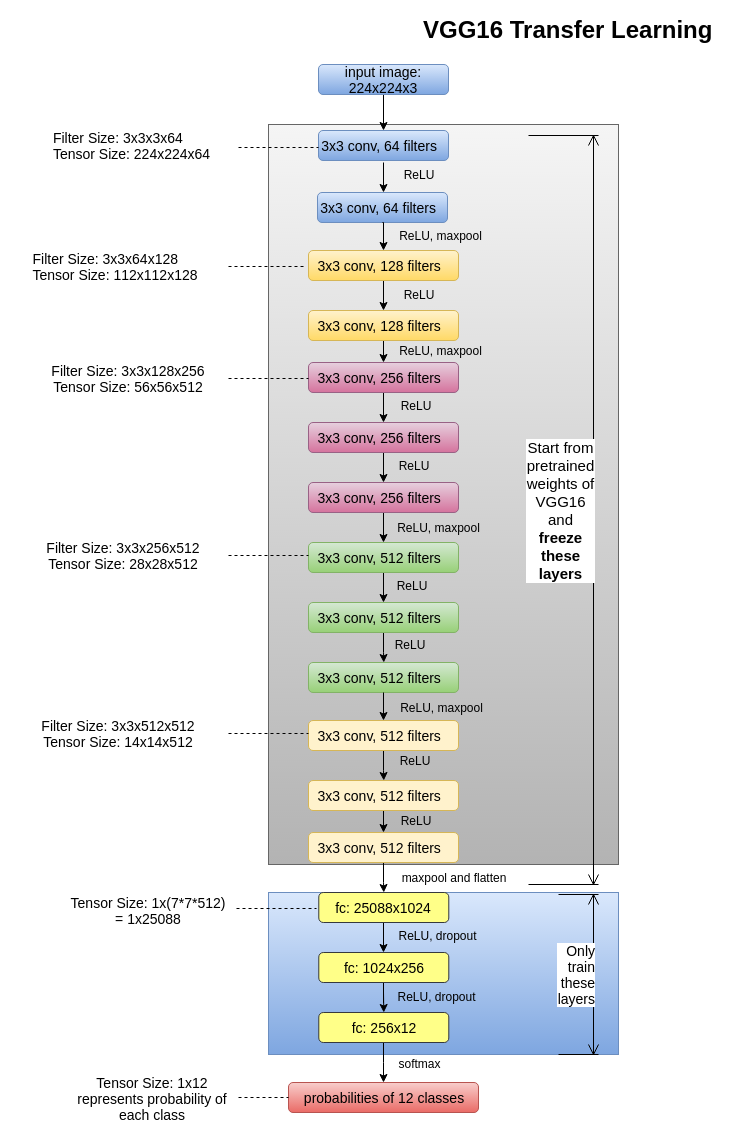
\includegraphics[width=0.9\hsize]{./figures/transferedVgg16}
	\caption{An example of transfer learning applied on VGG16 model. Note that the fully connected part was modified compared to the original VGG16. In addition there are only 12 categories to classify here.}
	\label{fig:transferedVgg16}
\end{figure}


\section{Object Detection}
\label{sec:objDetect}
\subsection{Problem Description}
The Image Classification problem presented in subsection \ref{sec:imgClass} is challenging, however, in reality, we are likely to deal with even more complex problem: the input image contains multiple objects. Furthermore, we would like to know where each object appears in the image. This task is named \textbf{Object Detection} and formally, it can be described as follows:
\begin{itemize}
	\item \tbf{Input}: An image that may contain multiple objects. Each object belongs to a finite set of classes.
	\item \tbf{Output}: The original image with predicted objects. Each object is surrounded by a predicted bounding box.
\end{itemize}
By solving this problem, we can detect multiple objects and also locate them in the image. Knowing the bounding box around the object helps us to estimate the distance from the camera to the objects. This is discussed in section \ref{sec:camModel}.

We see in the following subsections that the state-of-the-art solutions for Object Detection also rely on a robust image classifier. Hence doing well on Image Classification is a  prerequisite for a good object detection system.

\subsection{Evaluation}
The following notions (especially described in our context) are related to the evaluation of an object detection system:
\begin{itemize}
	\item A detection: a detection of our system is defined as an bounding box and a categorical distribution of the object in that bounding box. The object's label is chosen by the highest probability in that distribution.
	\item Intersection over Union (IoU): IoU of two bounding boxes $B_1$ and $B_2$ is defined by: $$IoU(B_1, B_2) := \frac{area(B_1 \cap B_2)}{area(B_1 \cup B_2)}$$
	\item Detection Validity: a detection with bounding box $B_p$ is considered \tbf{valid} if there exists at least one ground truth bounding box $B_{gt}$ such that $IoU(B_p, B_{gt}) \geq 0.5$
	\item True Positive $T_p$: a detection is marked as \tit{true positive} if it is the first valid detection with correct predicted label.
	\item False Positive $F_p$: any detection will be marked as \tit{false positive} if one of the following cases happens:
	\begin{enumerate}
		\item invalid detection (see definition for \tit{valid detection} above)
		\item valid detection with wrong predicted label
		\item valid detection with correct predicted label but there already exists a true positive for this ground truth bounding box
	\end{enumerate}
	\item False Negative $F_n$: a ground truth bounding box will be marked as one \tit{false negative} if there is no predicted bounding box that is valid for this ground truth bounding box
	\item Precision: $P = \frac{T_p}{T_p + F_p}$. 
	\item Recall: $R = \frac{T_p}{T_p + F_n}$ . Note that precision and recall are computed for each class in order to measure system's performance by class.
	\item Precision/Recall curve: we run the system through the test dataset once. For each image, we accumulate the precision and recall (for each class) computed so far and save these accumulated vectors. Once the detection system finishes, we use these accumulated vectors to plot precision corresponding to different recall levels.
	\item Average Precision (AP) for each class: to evaluate the system we use a metric called \tbf{Average Precision} that is defined below:
	$$ AP = \sum_k (R_k - R_{k-1})P_k $$
	where $P_k$ and $R_k$ are the precision and recall at the $k$-th recall level.
	\item mean Average Precision (mAP): is the averaged AP over all classes.
\end{itemize}
Remember that there could be multiple objects located arbitrarily in each image. A high precision ($F_p << T_p$) and low recall ($F_n >> T_p$) system will detect very few objects but most of its predictions are correct. On the other hand, a low precision ($F_p >> T_p$) and high recall ($F_n << T_p$) system will detect a lot of objects but most of its predictions are incorrect. Therefore, a good detector has to have both high precision and high recall. The metric Average Precision (AP) is chosen because it summarises the shape of the precision/recall curve (it is approximately the area under the precision/recall curve). A high area under the curve means both high precision and high recall. Since precision and recall are numbers in range $[0.0, 1.0]$, average precision (AP) will also be in this range and a higher AP is better.

\tbf{Remark:} there are various versions of the Average Precision calculation because people working in different domains (information retrieval, recommender system, computer vision etc.) adjust this metric to evaluate more appropriately their domain-specific tasks. We will use the general version defined above because this is the one used by the authors of Faster-RCNN method \cite{vocEval}. A version \cite{Everingham2010} that involves interpolation is used in PASCAL VOC challenges \cite{Everingham2010}. PASCAL VOC was a well-known annual competition in image classification, object detection and image segmentation in period 2005-2012. Although the challenge has finished but the PASCAL VOC dataset is still in extensive use today. We will use PASCAL VOC dataset to verify the correctness of the implementation. From figure \ref{fig:rcnnCompair}, we see that Faster-RCNN method scores around 70 mAP for VOC 2007 test dataset.

Given the Average Precision for each class, we can compute \tbf{mean Average Precision} across classes. This number will represent the system performance.

\subsection{State-of-the-art Solutions}
Faster-RCNN \cite{DBLP:journals/corr/RenHG015} is currently one of the best solutions for the Object Detection problem. It is based entirely on a convolutional neural network (\ref{fig:fasterRCNNfull}). We will also see related previous works (RCNN \cite{DBLP:journals/corr/GirshickDDM13} and Fast-RCNN \cite{DBLP:journals/corr/Girshick15}) to fully understand the method.

\subsubsection{RCNN}
The general idea to solve Object Detection problem is as follows: for each image
\begin{itemize}
	\item Step 1: Extract \tbf{\tit{regions of interest}} (\tbf{RoIs}) that have a high chance of containing objects. This step is also called \tbf{\tit{region proposals}}.
	\item Step 2: "Wrap" (i.e. resize) these regions (to have appropriate dimensions) and put these regions into a classifier to get the object label and adjust the bounding boxes accordingly.
	\item Step 3: With predicted probabilities from step 2, remove redundant regions. This method is called non-maximum suppression (see section 7.2 in \cite{Felzenszwalb:2010:ODD:1850486.1850574} for more details). Briefly, among the highly overlapped regions (greater than a overlap rate around $90\%$), we only keep the ones having highest probability.
\end{itemize}

Figure \ref{fig:rcnn} illustrates the R-CNN method (Regions with Convolutional Neural Networks features) \cite{DBLP:journals/corr/GirshickDDM13}. It uses an algorithm called Selective Search \cite{Uijlings:2013:SSO:2509349.2509382} to extract RoIs.
\begin{figure}[tb]
	\centering
	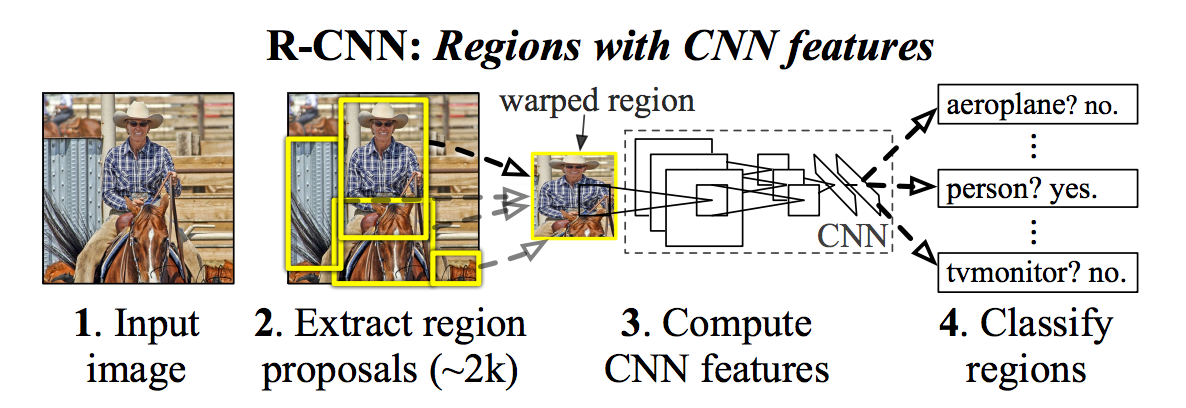
\includegraphics[width=1.0\hsize]{./figures/rcnn}
	\caption{Regional with Convolutional Neural Networks features: RoIs are extracted from Selective Search algorithm \cite{Uijlings:2013:SSO:2509349.2509382} and are wrapped (i.e. resized) to feed in a convolutional neural network. Image source: \cite{DBLP:journals/corr/GirshickDDM13}}
	\label{fig:rcnn}
\end{figure}
From figure \ref{fig:rcnn}, we can see the core engine of R-CNN is the convolutional neural network layers and the classifier on top of that. Hence, doing well in Image Classification is a need to perform well in Object Detection.

\subsubsection{Fast-RCNN}
The R-CNN method is really intuitive and straight-forward. However, it has a problem: it has to pass numerous RoIs to the network, and for overlapped regions the computation is repeated many times. Therefore, a more robust version of R-CNN: Fast-RCNN \cite{DBLP:journals/corr/Girshick15} passes the whole image to the CNN \tbf{once}, and extracts from that last layer the corresponding RoIs. These RoIs will pass through a RoI pooling layer to be given an appropriate dimensions. Now these RoI feature vectors are input of the classifier and a bounding box regressor. This is illustrated in figure \ref{fig:fastRCNN}. Note that each bounding box is represented by 4 coordinates $x_1, y_1, x_2, y_2$ which are positions of 2 corners top-left and bottom-right. The bounding box regressor is just a fully-connected layer ($out = W\times in + b$) that is applied on the ROI feature vectors to get the adjusted 4 coordinates accordingly.
\begin{figure}[tb]
	\centering
	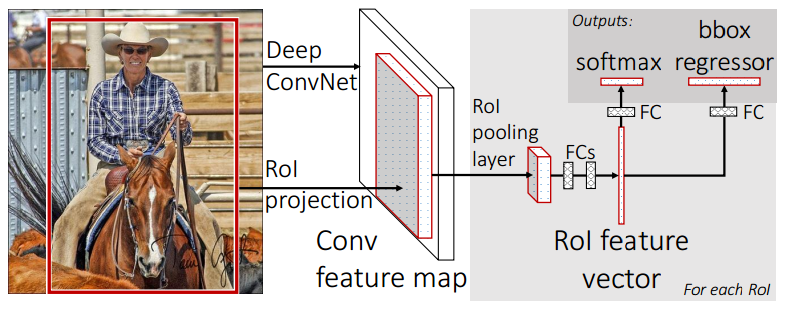
\includegraphics[width=0.9\hsize]{./figures/fastRCNN}
	\caption{\tbf{Fast-RCNN} (Fast Regional with Convolutional Neural Networks features): RoIs are projected from the last convolutional layer (i.e. the convolutional feature map) and are pooled to feed the classifier and bounding box regressor. Note that the RoIs on the original image are computed by Selective Search. Image source: \cite{DBLP:journals/corr/Girshick15}}
	\label{fig:fastRCNN}
\end{figure}

\subsubsection{Faster-RCNN}
Fast-RCNN is already good however there is one last bottleneck in the region proposal step. For a single image, it takes $\approx$ 2 seconds to run Selective Search while other computations can be done in $\leq$ 0.5 second (thanks to GPU for fast matrix calculation). Figure \ref{fig:rcnnCompair} illustrates this point. Hence, the \tbf{Faster-RCNN} method \cite{DBLP:journals/corr/RenHG015} integrates the region proposal step to the whole network by creating the \tbf{\tit{Regional Proposal Network}} \tbf{(RPN)} (figure \ref{fig:fasterRCNNfull}). RPN proposes k anchor boxes of different sizes and width/height ratios. For each anchor box, the RPN will detect whether it contains an object (\tit{cls} layer) and refine its shape and position (\tit{reg} layer). Remember that each bounding box is described by 4 coordinates: $(x_{min}, y_{min}, x_{max}, y_{max})$ - the positions of the top-left and the bottom-right corners.

\begin{figure}[tb]
	\centering
	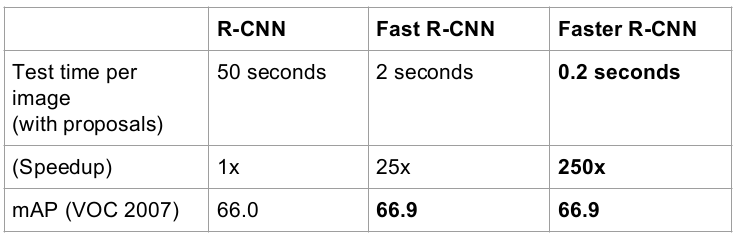
\includegraphics[width=0.8\hsize]{./figures/rcnnCompair}
	\caption{Speed and performance of RCNN, FastRCNN, FasterRCNN models in test time. Testing data is the Pascal VOC 2007 test set. Image source: \cite{cs231n}}
	\label{fig:rcnnCompair}
\end{figure}

\begin{figure}[tb]
	\centering
	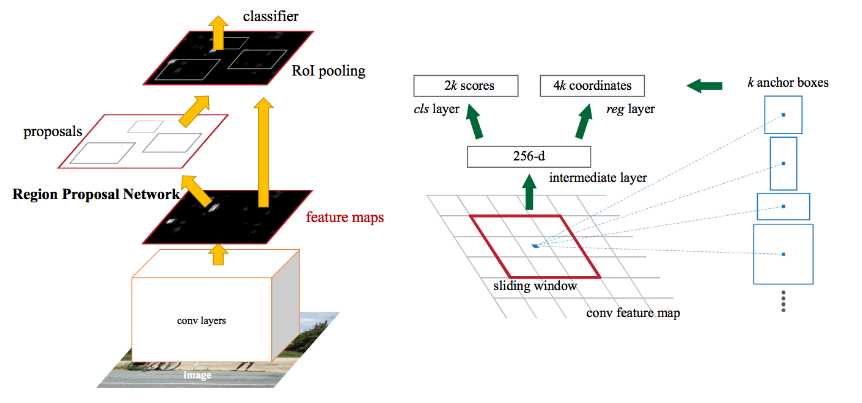
\includegraphics[width=1.0\hsize]{./figures/fasterRCNNfull}
	\caption{\tbf{Left}: Faster-RCNN integrates region proposal step to the whole network by creating Region Proposal Network (RPN). \tbf{Right}: RPN proposes k anchor boxes of different sizes and width/height ratios. For each anchor box, the RPN will detect whether it contains an object (\tit{cls} layer) and refine its shape and position (\tit{reg} layer). Image source: \cite{DBLP:journals/corr/RenHG015}}
	\label{fig:fasterRCNNfull}
\end{figure}

\subsubsection{A note on training}
The Faster-RCNN model has finally 4 loss functions (figure \ref{fig:lossFasterRCNN}). These 4 losses will be Let's denote the losses in RPN \tit{the lower head}; the losses in the final layer \tit{the upper head} respectively. There exists multiple training schemes as described in \cite{DBLP:journals/corr/RenHG015}. We will adopt the approximate joint training scheme which is simpler to implement and still gives similar performance to other schemes. The approximate joint training scheme is described as follows: 
For each gradient descent iteration
\begin{itemize}
	\item In forward pass: region proposals are treated as fixed, pre-computed proposals to train the upper head of the model.
	\item In backward pass: gradients flow as usual from both upper and lower head. 
	\item It is approximate because we do not calculate derivates of upper losses with respect to the region proposals' coordinates (since we are considering them fixed).
\end{itemize}
In addition, all the losses are defined mathematically in \cite{DBLP:journals/corr/RenHG015}. For more details, please refer to that paper.

\begin{figure}[tb]
	\centering
	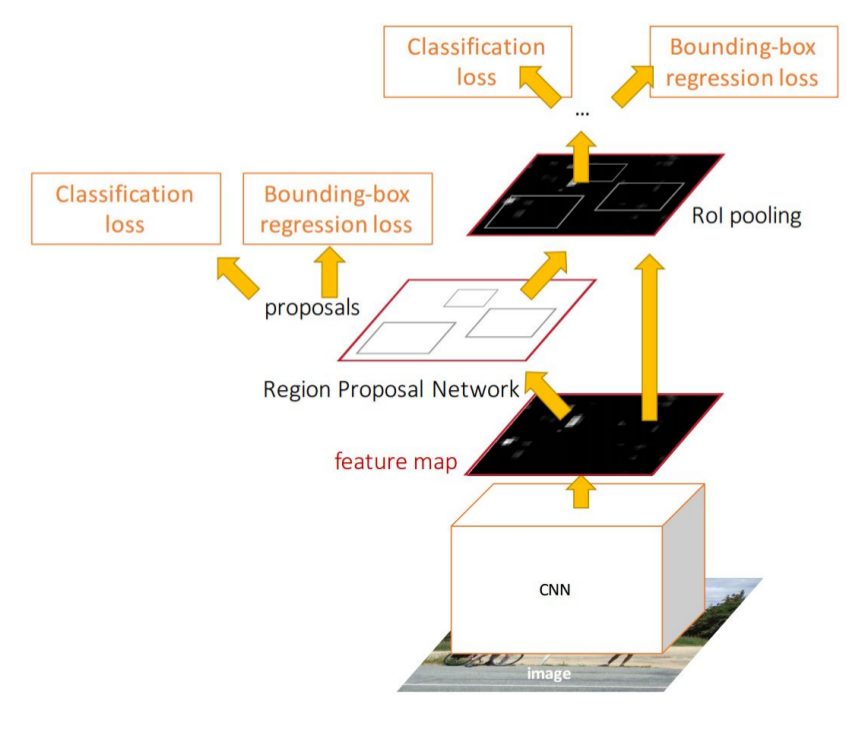
\includegraphics[width=0.8\hsize]{./figures/lossFasterRCNN}
	\caption{A 4-losses training pipeline. Image source: \cite{cs231n}}
	\label{fig:lossFasterRCNN}
\end{figure}

Based on the speed and robustness of Faster-RCNN method (figure \ref{fig:rcnnCompair}), I chose Faster-RCNN method to build our object detection system.


\section{Camera Model and Distance Estimation}
\label{sec:camModel}
\subsection{Overview}
We can estimate the distance from camera to objects if these three requirements are met: 
\begin{itemize}
	\item We have the ability to detect objects and neatly locate them in the image by surrounding a bounding box. By doing that we know the size (in pixels) of the area that the objects occupy.
	\item The camera's intrinsic parameters (focal lengths, image center, etc.) are known.
	\item The (estimated) size of the objects (in centimetres for example) are known.
\end{itemize}
Thourghout this section, we will see how the statement above applies. 

\subsection{Camera Model}
The robot's specification will be introduced more carefully in section \ref{sec:Cozmo}. I only note here that the robot's camera resolution is quite low ($320 \times 240$) and its field of view is also small ($\approx 50 ^{\circ}$). Based on these numbers, I chose to use a simple pinhole camera model that does not involve undistortion. An illustration of the model is shown in figure \ref{fig:pinhole} where $(u, v)$ are \tit{pixel coordinates on the image} and $(x,y,z)$ represent object's position \tit{in the camera's frame}.

\begin{figure}[tb]
	\centering
	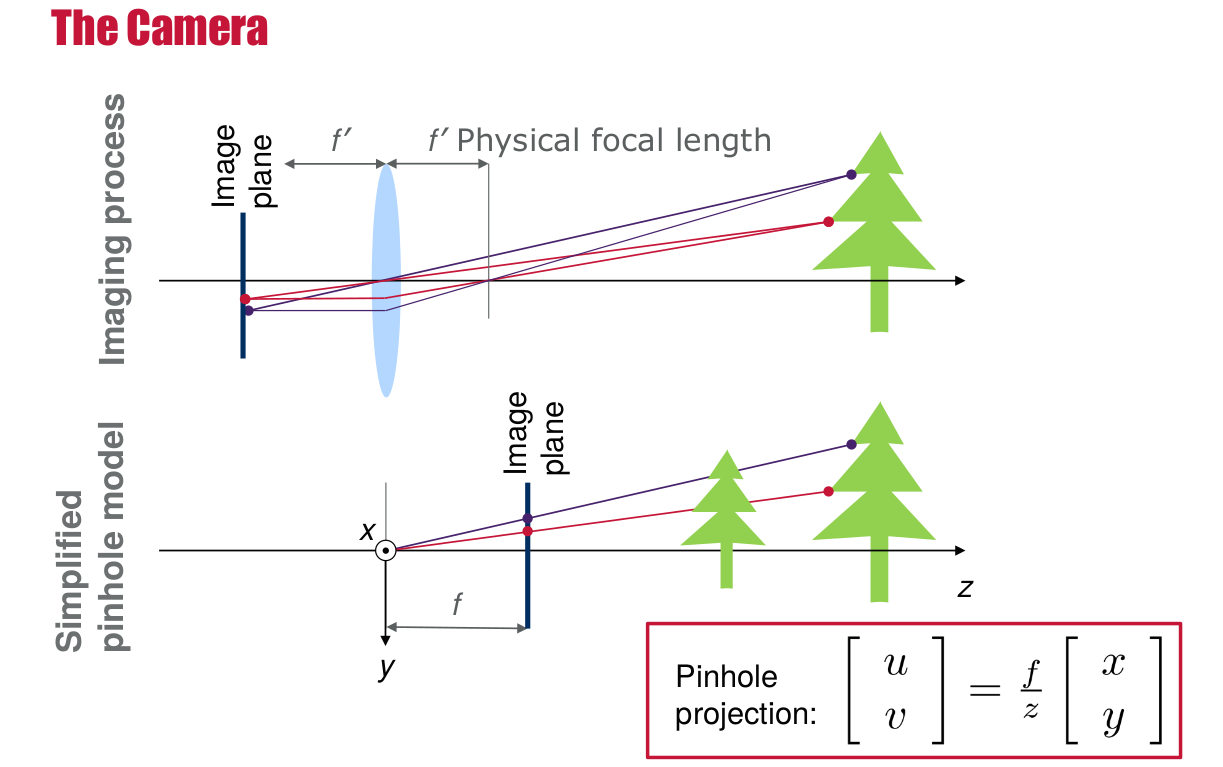
\includegraphics[width=0.9\hsize]{./figures/pinhole}
	\caption{Pinhole camera model: note that $(u, v)$ are pixel coordinates on the image, $(x,y,z)$ represent object's position in camera's frame. Image source: \cite{c433}}
	\label{fig:pinhole}
\end{figure}

In general, we have to take into account that the focal-lengths might differ and the origin of pixel coordinates is the top left corner of the image. Thus, the mathematical formula of the model is the following:
\begin{align}
	\label{form:pinhole}
\begin{bmatrix}
	u \\
	v
\end{bmatrix} = \begin{bmatrix}
f_1 & 0 \\
0 & f_2 
\end{bmatrix} \begin{bmatrix}
x/z\\
y/z
\end{bmatrix} + \begin{bmatrix}
c_1 \\ c_2
\end{bmatrix}
\end{align}

\subsection{Distance Estimation}
Let's go further by considering a rectangle which is parallel to the image plane at distance $z$. The top-left and bottom-right corners of rectangular are represented in the camera's frame by $(x_1, y_1, z)$ and $(x_2, y_2, z)$ respectively (figure \ref{fig:rectForm}). We can compute the width and height of the rectangle from these coordinates: $w = x_2 - x_1$, $h = y_2 - y_1$. Beside, from formula \ref{form:pinhole}, we have:
\begin{align}
	\label{form:dist0}
	\begin{bmatrix}
		u_1 \\
		v_1
	\end{bmatrix} = \begin{bmatrix}
	f_1 & 0 \\
	0 & f_2 
\end{bmatrix} \begin{bmatrix}
x_1/z\\
y_1/z
\end{bmatrix} + \begin{bmatrix}
c_1 \\ c_2
\end{bmatrix}
\hspace{0.5cm} \text{and} \hspace{0.5cm}
	\begin{bmatrix}
		u_2 \\
		v_2
	\end{bmatrix} = \begin{bmatrix}
	f_1 & 0 \\
	0 & f_2 
\end{bmatrix} \begin{bmatrix}
x_2/z\\
y_2/z
\end{bmatrix} + \begin{bmatrix}
c_1 \\ c_2
\end{bmatrix}
\end{align}

We then deduce:
\begin{align}
	\begin{bmatrix}
		u_2 - u_1\\
		v_2 - v_1
	\end{bmatrix} &= \begin{bmatrix}
	f_1 & 0 \\
	0 & f_2 
\end{bmatrix} \begin{bmatrix}
(x_2 - x_1)/z\\
(y_2 - y_1)/z
\end{bmatrix} \nonumber\\
\label{form:dist1}
\rightarrow u_2 - u_1 &= f_1 \frac{x_2 - x_1}{z} \hspace{0.5cm} \text{and} \hspace{0.5cm} v_2 - v_1 = f_2 \frac{y_2 - y_1}{z} 
\end{align}

\begin{figure}[tb]
	\centering
	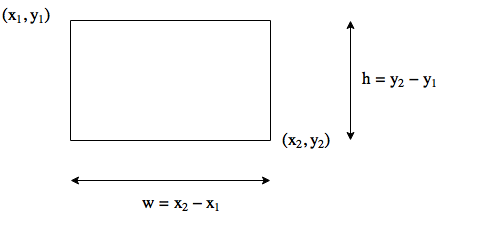
\includegraphics[width=0.6\hsize]{./figures/rectForm}
	\caption{A rectange at distance $z$ with top-left and bottom-right corners are represented in the camera's frame by $(x_1, y_1, z)$ and $(x_2, y_2, z)$ respectively. We deduce the width and height of this rectangle from the coordinates.}
	\label{fig:rectForm}
\end{figure}

Note that the image of this rectangular is also a rectangular with width and height in pixel coordinates are: $w_{i} = u_2 - u_1$, $h_{i} = v_2 - v_1$. Combine this with formula \ref{form:dist1} we have:
\begin{align}
\label{form:dist2}
z = f_1  \frac{w}{w_i} \nonumber \\
z = f_2  \frac{h}{h_i}
\end{align}
In reality, these two function will not return a same result because of the measure errors as well as the simplicity of the camera model. Hence we could compute the average:
\begin{align}
z = \frac{1}{2} (f_1 \frac{w}{w_i} + f_2 \frac{h}{h_i})
\label{form:distEst}
\end{align}

Given the real size of the rectangle ($w, h$), the camera's information ($f_1, f_2$) and the image size of the rectangle ($w_i, h_i$), we can deduce the distance $z$. Now, given $z$ computed, we plug it into formula \ref{form:dist0} together with information of the image center ($c_1, c_2$), we can easily derive the position $(x_1, y_1, x_2, y_2)$ of the rectangle:
\begin{align}
	x_1 = \frac{(u_1 - c_1)z}{f_1} \hspace{0.6cm}
	x_2 = \frac{(u_2 - c_1)z}{f_1} \hspace{0.6cm}
	y_1 = \frac{(v_1 - c_2)z}{f_2} \hspace{0.6cm}
	y_2 = \frac{(v_2 - c_2)z}{f_2} 
\end{align}
And then deduce the center of the bounding box:
\begin{align}
	\label{form:centerIm}
x_c = \frac{1}{2}\frac{(u_1 + u_2 - 2 c_1)z}{f_1} \hspace{0.5cm} y_c = \frac{1}{2}\frac{(v_1 + v_2 - 2 c_2)z}{f_2}
\end{align}
All the camera's information mentioned above (focal lengths, image center) can be obtained by doing camera calibration. Fortunately, these specifications are provided by the robot manufacturer (accessed by SDK they provide \cite{ANKI:2017}). Those details will be mentioned in section \ref{sec:Cozmo}.
This distance estimation capability enables a variety of actions such as localization of the robot in a map with some known fixed tags or autonomous path planning to reach objects.
\subsection{Error Estimation}
In reality, we need to take into account the errors of camera sensor, predicted bounding box, perspective view and size variance of objects. Let's find out the mathematical formula of this error, in a simple experiment, where we estimate distance from a cube placed parallel to the image plane to the camera. In addition, our camera has identical focal length $f_1 = f_2$ (see subsection \ref{subsec:camInfo}). Let's denote $f = f_1 = f_2$ the focal length. Let's also assume the cube is close to the center of image (i.e. on the $z$ axis). Hence the distance from the camera is approximately the $z$ value from formula \ref{form:dist2}. By taking total derivative of formula \ref{form:dist2} we have:
\begin{align*}
& \hspace{0.3cm} z = f \frac{h_i}{h} \\
&\rightarrow \ln z = \ln f + \ln h_i - \ln h \\
&\rightarrow \frac{d z}{z} = \frac{d f}{f} + \frac{d h_i}{h_i} - \frac{d h}{h}
\end{align*}
Let's denote $\Delta x$ the absolute error estimation of parameter $x$. We have the relative error estimation:
\begin{align}
\frac{\Delta z}{z} =  \frac{\Delta f}{f} + \frac{\Delta h_i}{h_i} + \frac{\Delta h}{h}
\label{form:errEst}
\end{align}
We can see from formula \ref{form:errEst} that the relative error is big if: 
\begin{itemize}
	\item object is small ($h$ is small)
	\item object is far from the camera ($h_i$ is small)
	\item bounding box is not accurate ($\Delta h_i$ is big)
	\item camera has low resolution (upper bound of $h_i$ is small)
	\item object has big size variance ($\Delta h$ is big)
\end{itemize}
We will revise these above statements in section \ref{sec:distEstimExp}, where we really setup the experiment and estimate distance from the robot to a cube.

%\subsection{Error Estimation}
%Given the formula \ref{form:distEst}, we want to know the error $\Delta z$ when we compute the distance $z$. This can be obtained from the total derivative form:
%\begin{align*}
%dz = \frac{1}{2} \bigg( \frac{\partial z}{\partial f_1}df_1 + \frac{\partial z}{\partial f_2}df_2 + \frac{\partial z}{\partial f_1}df_1 + \frac{\partial z}{\partial f_1}df_1     \bigg)
%\end{align*}